%============================ 5. DISCUSSION ===================================
\isec{\faComments}{Discussion}
\label{sec:discussion}

\isub{\faEquals}{Consistency of the trials}
The ten errors lie between $-0.48$ and $+0.48$\,cm, with a standard deviation of 0.32\,cm and a mean of
$-0.10$\,cm. The mean is smaller than its own standard error ($0.32/\sqrt{10}=0.10$\,cm), so there is no evidence of a
systematic offset: the remaining error is scatter, not bias.

Where the robot \emph{stopped} varied much more than how well it \emph{knew} where it stopped. The tape readings range
from 0.480 to 0.498\,m: in trials 5 to 8 the robot coasted 1.4 to 2.2\,cm past the brake point after the speed command went
to zero. The estimate followed this coasting in every case (correlation 0.90 between $d_{est}$ and $d_{meas}$), so the
stopping error belongs to the controller and the chassis, not to the estimator. Stopping more precisely would need a
lower final speed or braking earlier; it would not change the estimation error that this project measures.

\isub{\faSearch}{Sources of error}
\begin{table}[H]
\centering\small
\setlength{\tabcolsep}{4pt}
\rowcolors{2}{kfupmlight}{white}
\begin{tabularx}{\linewidth}{@{}>{\raggedright\arraybackslash}p{3.2cm}>{\raggedright\arraybackslash}X>{\raggedright\arraybackslash}p{3.6cm}@{}}
\rowcolor{kfupm}\hd{Source} & \hd{Evidence in this project} & \hd{Effect and handling}\\
Wheel slip on the rug & odometry over-reads the travel by 1.5 to 2.1\,\% (both calibration runs) & along-track drift; corrected by the camera range\\
Odometry glitches & 10 impossible pose steps in trials 6, 8, 9, 10; wheels-only error 2.9 to 5.8\,cm there & guard skips them; camera removes the lost travel\\
\code{/odom} twist field & 20 to 40\,\% too high and over 1\,s late; 38\,cm error in test 1 & not used; speed from the pose\\
Camera range calibration & fit through two tape anchors; check points within 3 and 7\,mm & residual bias, shared by EKF and camera (both $\approx$0.3\,cm)\\
Camera detection limits & tag 10\,px tall at 1.5\,m (unreliable), lost below 0.47\,m & start 1.20\,m, stop 0.50\,m\\
Camera outliers & 8 readings with NIS $>$ 9.21 in trial 9 & $\chi^2$ gate\\
Wi-Fi drops & 3\,s drop in calibration: robot kept moving 14\,cm, \code{/odom} reset & none in the 10 trials; such a trial would be repeated\\
Tape reading & read to about $\pm$2 to 3\,mm from the chassis front & of the same size as $\sigma=3.2$\,mm\\
Controller coasting & 1.4 to 2.2\,cm past the brake point in trials 5 to 8 & stopping error, tracked by the estimate\\
\end{tabularx}
\caption{Error sources, each with the evidence for it.}
\label{tab:sources}
\end{table}

The final error of 0.28\,cm is about the size of the tape reading uncertainty, so the result should be read as
\emph{the estimate agrees with the tape to within the resolution of the tape}, not as millimetre accuracy.

\isub{\faBalanceScaleLeft}{Role of prediction and correction}
\label{sec:role}
To separate what each part contributes, the logged inputs of the 10 trials were fed again through the same
\code{RobotEKF} code with one ingredient removed (\code{scripts/replay_ekf.py}). Replaying the unchanged filter
reproduces the logged estimate to within 0.04\,mm, so the differences below are caused only by the removed ingredient.

\begin{table}[H]
\centering\small
\rowcolors{2}{kfupmlight}{white}
\begin{tabular}{@{}lrrrr@{}}
\rowcolor{kfupm}\hd{Filter variant (same 10 trials)} & \hd{MAE (cm)} & \hd{bias (cm)} & \hd{$\sigma$ (cm)} & \hd{worst $|e|$ (cm)}\\
\textbf{As run: prediction + odometry + camera range and bearing} & \textbf{0.28} & $-0.10$ & 0.32 & 0.48\\
Camera noise $R_{tag}\times3$ & 0.25 & $+0.16$ & 0.31 & 0.68\\
Camera noise $R_{tag}/3$ & 0.30 & $-0.13$ & 0.34 & 0.54\\
Camera only, last reading, no filter & 0.30 & $-0.15$ & 0.33 & 0.55\\
Camera lost below 0.90\,m (prediction carries the last 40\,cm) & 1.86 & $+1.17$ & 1.64 & 2.72\\
Camera bearing only, no range & 1.98 & $-0.95$ & 2.63 & 4.92\\
No camera while driving (prediction + odometry) & 2.53 & $-1.52$ & 3.12 & 6.20\\
\end{tabular}
\caption{Offline replay: final-distance error with parts of the filter removed (\code{results/replay/}).}
\label{tab:replay}
\end{table}

\begin{figure}[H]
\centering
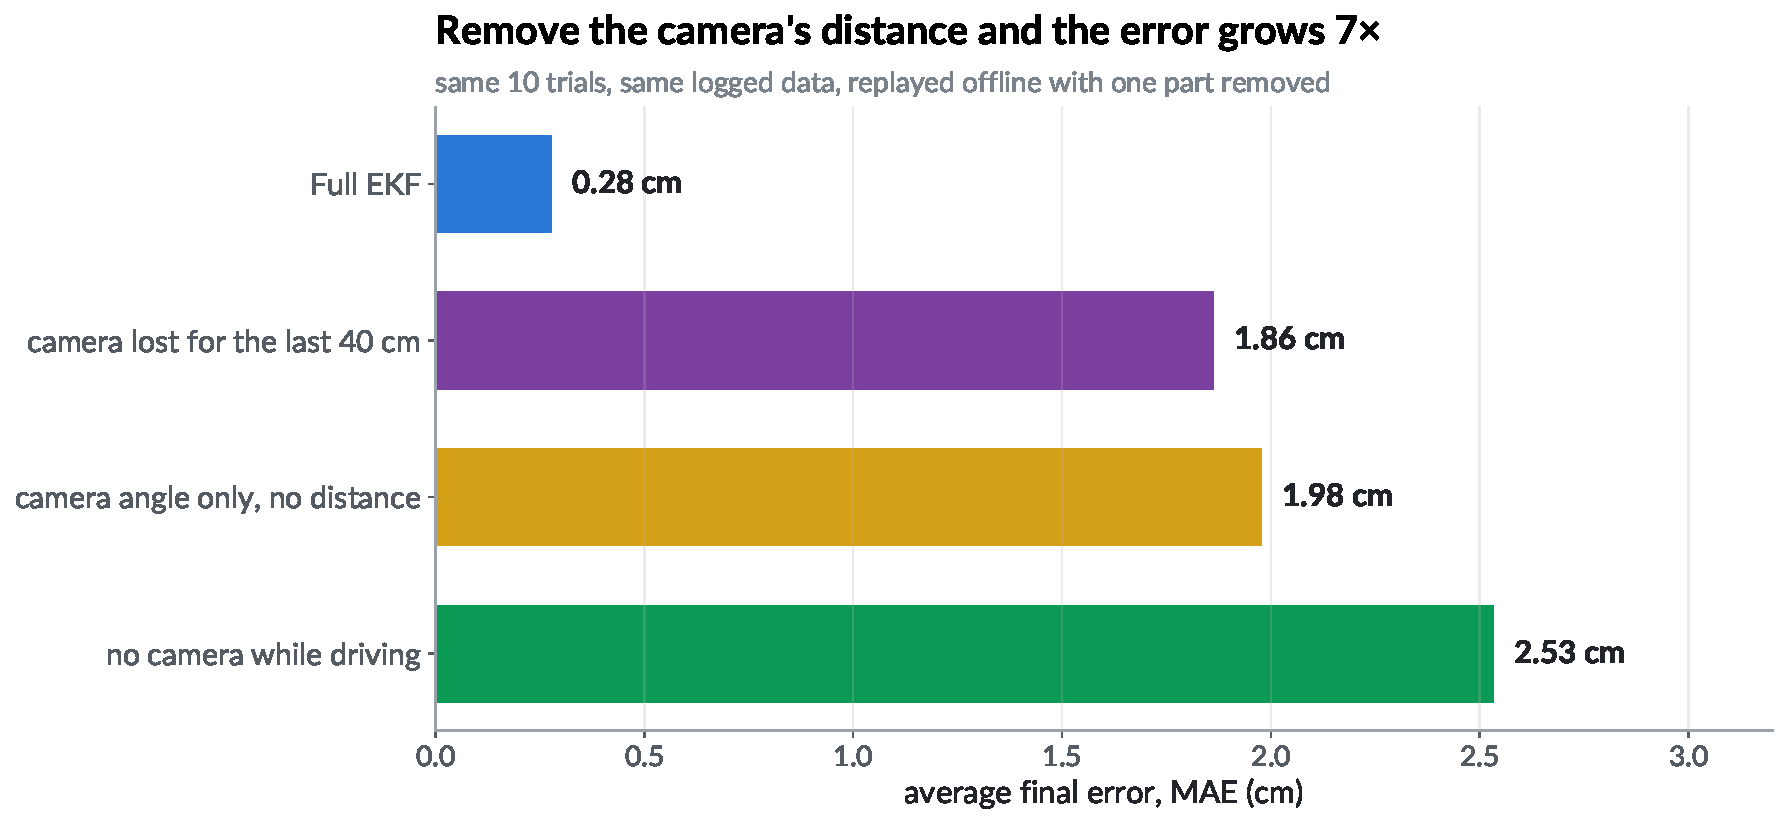
\includegraphics[width=0.86\linewidth]{figures/simple_6_contrib.pdf}\\[6pt]
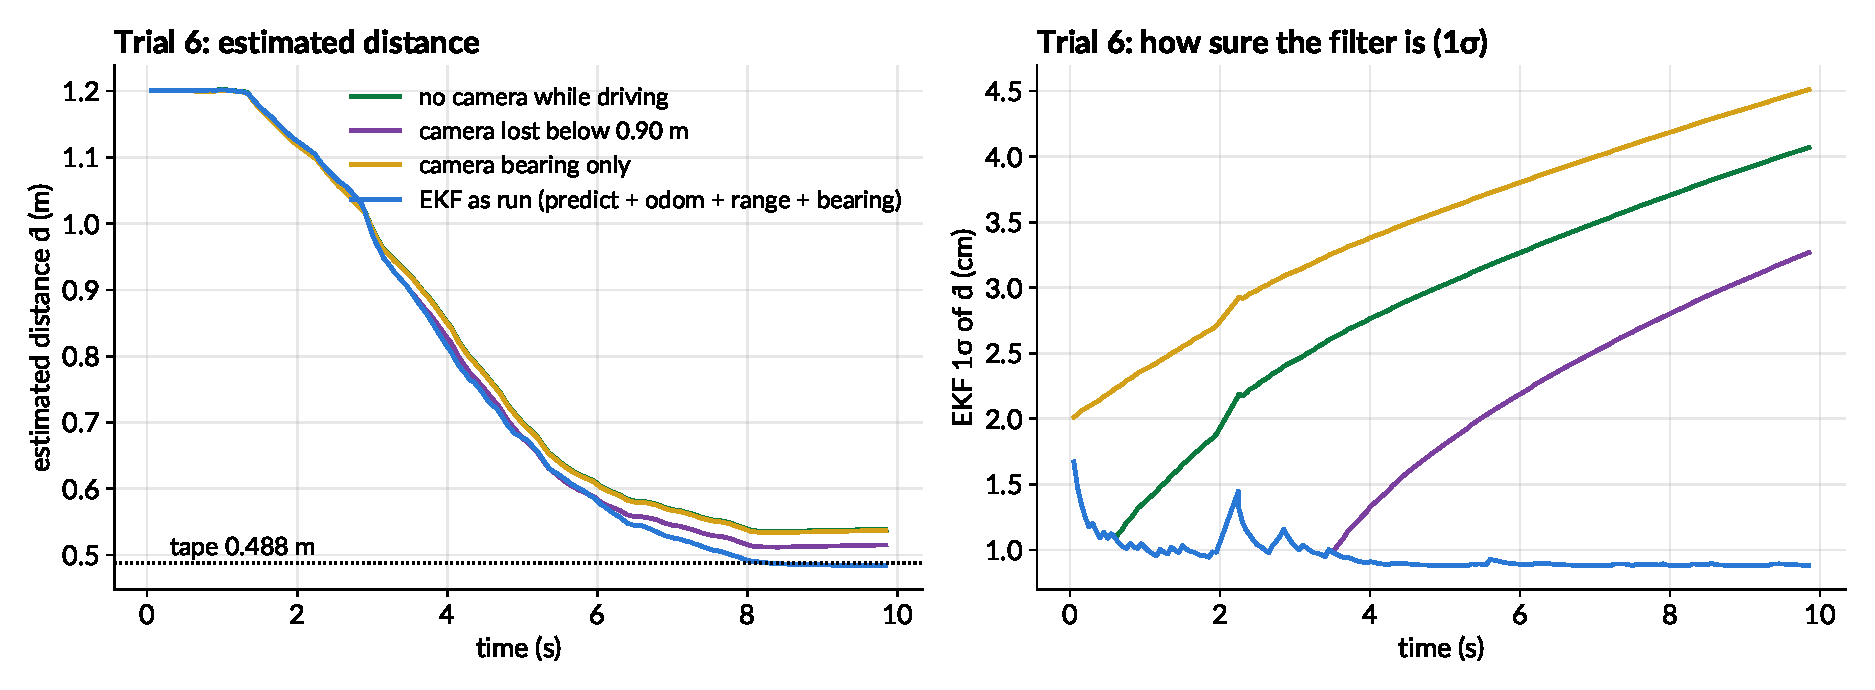
\includegraphics[width=0.92\linewidth]{figures/fig_replay_trial6.pdf}
\caption{Top: average final error when one part of the filter is removed. \textbf{How to read it:} shorter is better;
each bar is the same 10 trials replayed. Bottom: trial 6 replayed. Without the camera (green) the estimate drifts away
from the tape and its uncertainty $\sigma_d$ keeps growing; with the camera (blue) every correction pulls it back and
keeps $\sigma_d$ below 1\,cm.}
\label{fig:replay6}
\end{figure}

\lead{Prediction.} The motion model with odometry gives a smooth estimate at 20\,Hz, between camera fixes and through
any gap. On its own it is not enough: with no camera while driving the final error grows to 2.5\,cm on average and
6.2\,cm in the worst trial, and $\sigma_d$ grows with the distance driven (Figure~\ref{fig:replay6}). Two kinds of
odometry error cause this: slow drift from slip (about 1.5 to 2\,\% of the distance) and sudden glitches. Prediction is
also what makes the correction safe: the gate can reject a bad camera reading only because the prediction says where
the tag should be.

\lead{Correction.} The camera range bounds the along-track error at every fix, so the final error does not depend on
how far the robot drove or on how many odometry steps were lost. Trial 6 shows this directly: the wheels alone end
5.8\,cm off, the EKF 0.4\,cm.

\lead{Why range is required (Lecture 12A, slide 26).} Driving straight at the tag, $\Delta y\approx0$, so the bearing row
of $H_{tag}$ is $[\,0,\ -1/d,\ -1,\ 0,\ 0\,]$: its $p_x$ entry is zero, and bearing carries no information about the
distance along the line, which is exactly where odometry drifts. Only the range row $[-1,0,0,0,0]$ observes it.
The replay confirms it: bearing only gives 1.98\,cm, almost as bad as no camera at all (2.53\,cm), while range and bearing
give 0.28\,cm.

\lead{EKF versus the camera alone.} At the final position, the EKF (0.28\,cm) and the last camera reading (0.30\,cm) are
nearly equal. This is expected here, because the camera sees the tag until the stop, and the estimate at rest is
dominated by many camera fixes. The value of the filter is in what the camera alone cannot do: give an estimate at
every control tick with a known uncertainty, reject outliers, survive odometry glitches, and keep a usable estimate when
the camera is lost (1.86\,cm after 40\,cm without the camera, against no estimate at all).

\isub{\faHeartbeat}{Is the filter's uncertainty honest?}
\label{sec:consistency}
The filter reports $\sigma_d=0.90$\,cm at the stop, while the real spread is 0.32\,cm (ratio 0.36), and all 10 errors are
inside $\pm2\sigma_d$. The filter is therefore cautious rather than overconfident, which is the safe side: an overconfident
filter would start rejecting good camera readings at the gate. The replay with $R_{tag}\times3$ and $R_{tag}/3$ changes
the MAE by only 0.05\,cm, so the result does not hinge on the exact noise values. A tighter $R_{tag}$ (about 1\,cm
instead of 3\,cm) would bring $\sigma_d$ closer to the observed spread.

\isub{\faExclamationTriangle}{Limitations and transparency}
\begin{warnbox}
\small
\begin{itemize}
  \item \textbf{Two trials were repeated.} Trials 5 and 9 were run a second time after the first tape reading disagreed
        with the estimate by 12 and 10\,mm. Both first attempts are kept in \code{results/test_runs/} with their readings.
        If the first attempts are used instead, the MAE is 0.45\,cm, $\sigma$ = 0.59\,cm and the range $-1.19$ to
        $+0.99$\,cm; the conclusions do not change.
  \item \textbf{Same tape, same reference point.} The camera was calibrated against the same tape and reference point
        that later measured the trials, so the statistics measure repeatability and calibration residual rather than
        accuracy against an independent instrument.
  \item \textbf{Single geometry.} One start distance, one floor and one tag; the camera-limited stop at 0.50\,m was chosen
        for this tag size.
\end{itemize}
\end{warnbox}
